
    The research contributions of this thesis are based on a novel constraint
    programming approach on compiler intermediate representation.
    This chapter introduces the theoretical underpinnings of this approach,
    based on a mathematical model of static single assignment form (SSA).
    With the help of this model, concepts that are typically discussed on a
    programming language level are transferred onto the structurally simple,
    yet semtantically expressive class of SSA compiler intermediate
    representations.

    Constraint formulas on SSA respresentations initially appear to mimic
    pattern matching approaches on abstract syntax tree (AST) level.
    However, they quickly prove themselves to be vastly more expressive.
    Some consideration is necessary to handle search space explosion, but
    the reward are much more powerful recognition capabilities and the
    expression of higher level algorithmic structures, which are impossible to
    define syntactically on programming language level.
    Later chapters will explore the power of this approach in detail, by
    building a complete constraint programming language on top of the theory in
    this chapter, and by then using it to solve real compiler analysis problems.

    After defining a mathematical foundation of SSA form and introducing
    formalisms for the expression of basic contraint problems on top of it,
    several standard definitions from compiler theory are reformulated in the
    framework.
    This includes common graph properties, including the concept of domination,
    as well as control flow structures such as single entry single exit blocks.
    All of this lays the foundations for the succeeding chapter.

    Finally, for the practical application of constraint programming to compiler
    intermediate representation, efficient solver techniques are needed.
    The last section in this chapter discusses strategies for limiting
    compile time explosion and explores analogies of the described model to
    standard Satisfiability Modulo Theory (SMT) problems.
    This gives further insights into performance improvements and puts the
    work into a broader theoretical context.

\section{Introduction}

    Modern compilers for procedural languages such as
    C/C++, Fortran or JavaScript typically use a succession of different
    representations for the program during compilation.
    They can be grouped into categories and reflect the requirements of
    the compilation stages they are used in.
    \linebreak
    {\bf Front end representations} are close to the source program and
    naturally reflect the internals of the compiler front end, especially the
    parser.
    Typically, they are built on an abstract syntax tree representation with
    additional annotations, such as type information.
    In addition to encoding program logic, these representations are rich in
    information about syntactic and  stylistic choices of the programmer.
    They scale in complexity with the source language and further obscure the
    program semantics by not resolving complex language features, such as
    operator overloading.
    \linebreak
    {\bf Back end representations} are based on a model of the target hardware.
    These representations typically approach an assembly style format,
    exposing specific instruction set architectures of the hardware.
    Back end representations are concerned with problems that are removed from
    the algorithmic core of the user program, such as register allocation and
    instruction scheduling.
    \\
    {\bf Static Single Assignment} (SSA) form has emerged as a suitable
    representation in the middle end, which is traditionally responsible for
    applying complex optimising transformations.
    SSA abstracts away the complexities of both the source language and the
    target architecture, instead focusing on a relatively simple semantic
    description of the user program that enables reliable analysis and platform
    independent reasoning.
    It is these properties that also make it the natural representation for
    expressing algorithmic structures.

    Static Single Assignment is not a strictly defined or mathematically
    codified standard, but instead refers to a group of representations that
    share important characteristics,
    the eponymous SSA property being only one among them.
    Instruction sets, syntax and type systems of the different
    SSA intermediate representations vary considerably, depending on the
    requirements of the source languages (static or dynamic)
    and the operating constraints (just-in-time or ahead-of-time).
    Some prominent examples of compilers that utilize SSA for their
    optimisation passes include {\bf clang} (LLVM IR), {\bf gcc} (GIMPLE),
    {\bf v8 Crankshaft} (Hydrogen) and {\bf SpiderMonkey} (IonMonkey/MIR).
    Despite many differences, they share the same fundamental paradigms
    and many of the differences can be abstracted away as implementation
    specific details.

    Fundamentally, a program in single static assignment form is made up of
    functions, which are represented as sequences of instructions, grouped into
    basic blocks and operating on virtual registers.
    The control flow is handled via jump instructions at end of basic blocks.
    The virtual registers, within a function, can be assigned only at a single
    static location each, which has very useful implications as we will later
    see.
    As opposed to syntax-heavy representations, SSA form is a searialized
    program representation, where expressions have been turned into lists of
    instructions and control flow structures into lists of basic blocks.
    The following sections explore how this serial nature makes constraint
    programming concepts naturally applicable.

\subsection{Static Single Assignment Form}

\begin{figure}[t]
\centering
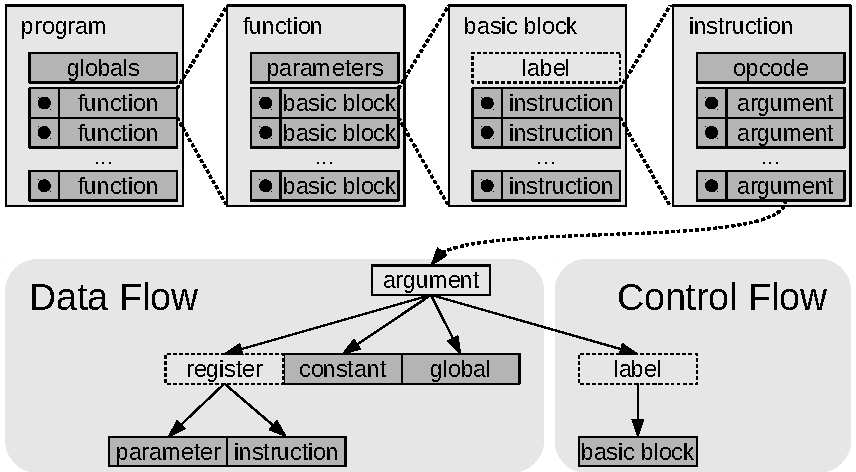
\includegraphics{figures/ssaoverview}
\caption{Structural overview of SSA: Programs are represented as hierarchies of
    lists. The SSA property makes registers implicit, values can be statically
    matched to defining instructions.}
\label{fig:ssaoverview}
\end{figure}

    SSA representations of programs are highly serialised, as shown in
    \autoref{fig:ssaoverview}:
    Programs are lists of functions, functions are lists of basic blocks,
    basic blocks are lists of instructions and instructions are most
    fundamentally lists of arguments.

    The individual instructions operate on an abstract machine, which provides
    an unlimited number of identical registers and a well defined instruction
    set.
    The control flow is expressed as branch instructions, which direct the
    execution conditionally or unconditionally to other basic blocks.
    Basic blocks may have labels or be identified simply by enumerating them.
    Instruction arguments can be registers, constants or globals and branch
    instructions additionally take basic block labels.
    Instructions can write their result into a single output register.
    Branch instructions always terminate a basic block, control flow divergence
    within basic blocks is not possible.

    The static single assignment property stipulates that within a function,
    no register can be written at more than a single static location.
    This makes the data dependencies between the instructions explicit, as it
    implies that registers can be identified directly with the instructions that
    write to them.
    The registers themselves can therefore be considered implicit, with only the
    data flow between instructions required to recover them.

    In the presence of dynamic control flow behaviour in the program, most
    simply in the case of a conditional branch, it is evidently not possible to
    match values to producing instructions statically.
    This is resolved with {\em phi} instructions.
    These instructions select a value from several arguments depending on the
    previously executed basic block, i.e.\ depending on the branch from where
    the execution reached the basic block containing the phi node.

\subsection{Example of Static Single Assignment Form}

    \autoref{ssaexample} shows many of the key features of static single
    assignment form and how they naturally emerge from simplification steps of
    the source code of procedural languages.
    This is demonstrated on an example C function ``{\tt sqrt}'',
    which  appriximates the square root of a double precision floating point
    value using the Babylonian method, as described in
    \autoref{babylonian_equation}.

\begin{equation}
    x_0\approx\sqrt{S},\text{\hspace{1cm}}
    x_{n+1}=\frac{x_n+\frac{S}{x_n}}{2}\text{\hspace{1cm}}
    \implies\text{\hspace{1cm}}
    \lim_{n\rightarrow\infty}x_n=\sqrt{S}
    \label{babylonian_equation}
\end{equation}

    Starting from the source code {\bf a)} at the top left of the figure, the
    function is first simplified by breaking down complex expressions as far as
    possible.
    This results in a sequentialisation of the expressions into their
    most basic operations, shown at the top right {\bf b)}, introducing
    explicit variables that store the previously implicit temporary values.
    This greatly simplifies and normalises the program, with many of the
    remaining simple expressions directly mapping to individual processor
    instructions.

    In a second step, the structured control flow of the program is replaced
    with goto statements that coordinate the control between basic blocks.
    This is shown at the bottom right {\bf c)}.
    While this does not ease the intuitive understanding of the program, it
    unifies the many control flow structures provided in the source language
    into a single mechanism.
    This makes automatic analysis of the program a less complex task.
    Importantly, no relevant information is lost by discarding the control flow
    structures.
    They can be reconstructed algorithmically.

    Lastly, the static single assignment property is introduced.
    Any variable that is assigned in more than one static place in the program
    is instead duplicated into multiple variables.
    Where necessary, these now distinct variables are bound together with
    $\Phi$ nodes.
    This cannot be directly expressed in the C syntax {\bf d)} at the bottom
    left.
    Instead, the behaviour is documented by comments in lines 8-13.
    The impact of the static single assignment property change seems minor
    at first, but it has convenient implications.
    As all local variables are written exactly once, the distinction between
    their declarations and definitions becomes obsolete.
    This furthermore implies that it is always known statically, which
    expression yielded the value of each variable.
    Variable names become identifiers of the expressions themselves.
    This makes many optimising transformation strainghtforward to implement.
    As a trivial example, it immediately guarantees that the variable $i$ in the
    example always has the value zero.

    With an understanding of how SSA form emerges during compilation, it is now
    the aim to use the serialised nature of it to contruct a convenient
    mathematical model.
    The crucial observation is that most items in SSA form functions can be
    easily enumerated and identified by their index.
    This includes the function parameters, expressions and variables.
    This means that properties of SSA form functions can be described using
    integers, making for a convenient and easy mathematical language.

\begin{figure}[p]
    \begin{minipage}{0.48\textwidth}
\begin{lstlisting}[language=C,captionpos=t,title=
   {{\bf(a)} {} C source function:\leftskip=0pt}]
double sqrt(double S) {
  double x = 1.0;
  for(int i=0; i<N; i+=1)
    x = 0.5 * (x + S / x);
  return x;
}
\end{lstlisting}
\begin{lstlisting}[language=C,captionpos=t,title=
   {{\bf(d)} {} The SSA property is introduced:\leftskip=0pt}]
double sqrt(double S) {
entry:
  double x = 1.0;
  int i = 0;
  goto header;

header:
  int i2 = /* if reached
    from line  5: i,
    from line 23: i3 */
  int x2 = /* if reached
    from line  5: x,
    from line 23: x3 */
  bool test = i2 < N;
  if(test) goto loop;
      else goto exit;

loop:
  double t1 = S / x2;
  double t2 = x2 + t1;
  double x3 = 0.5 * t2;
  int i3 = i2+1;
  goto header;

exit:
    return x2;
}
\end{lstlisting}
\end{minipage}
\hfill
\begin{minipage}{0.48\textwidth}
\begin{lstlisting}[language=C,basicstyle=\linespread{1.06451612903}\ttfamily,
                   captionpos=t,title=
   {{\bf(b)} {} Complex expressions are broken down:\leftskip=0pt}]
double sqrt(double S) {
  double x = 1.0;
  for(int i=0; i<N; i+=1)
  {
    double t1 = S / x;
    double t2 = x + t1;
    x = 0.5 * t2;
  }
  return x;
}
\end{lstlisting}
\begin{lstlisting}[language=C,basicstyle=\linespread{1.06451612903}\ttfamily,
                   captionpos=t,title=
   {{\bf(c)} {} Structured control flow is expanded:\leftskip=0pt}]
double sqrt(double S) {
entry:
  double x = 1.0;
  int i = 0;
  goto header;

header:
  bool test = i < N;
  if(test) goto loop;
      else goto exit;

loop:
  double t1 = S / x;
  double t2 = x + t1;
  x = 0.5 * t2;
  i = i+1;
  goto header;

exit:
    return x;
}
\end{lstlisting}
\end{minipage}

    \caption{Static Single Assignment emerges from successive simplification
             and normalisation of source language features: 
             Demonstration on an example C function that approximates the
             square root of an input value with the Babylonian method.
             The transformation results {\bf b)-d)} are redered in C.
             Real compilers typically operate on
             dedicated internal representations instead.}
    \label{ssaexample}
\end{figure}

\newpage
\section{Deriving a Mathematical Model for SSA}

    In order to develop constraint programming on real world SSA programs with
    mathematical rigour, a sound model is needed first.
    The aim here is not to introduce an operational semantics, or more
    generally to derive a model for the execution of SSA programs.
    Instead, the section will investigate the static structure, focusing on
    clear notation of the commonalities of existing SSA intermediate
    representations.
    This requires naming conventions for some of the basic features of
    SSA programs.
    The remainder of this section adheres to \autoref{not:ssa} when referring to
    these features.
    No specific representative of the class of SSA representations is chosen
    here.

\begin{figure}[h]
\begin{notation}{Static Single Assignment Function}{ssa}
    For the remainder of this section, some function $\mathcal F$ in SSA form is
    assumed fixed. 
    The following identifiers are then used to describe the features of this
    function.

    \begin{itemize}
    \item $|par|$ is the number of function parameters
          $par_1,\dots par_{|par|}$.
    \item $|ins|$ is the number of instructions $ins_1,\dots ins_{|ins|}$ in the
          function, ordered depth first, starting from the execution entry.
    \item $|glb|$ is the number of unique globals $glb_1,\dots glb_{|glb|}$ that
          are referenced as an operand of any of the instructions.
    \item $|cst|$ is the number of unique constants $cst_1,\dots cst_{|cst|}$
          that are referenced as an operand of any of the instructions.
    \end{itemize}
\end{notation}
\end{figure}

    This notation fixes several decisions about the utilised model.
    Firstly, the model captures only a single function.
    Secondly, basic block structures are not explicitly encoded.
    Instead, all instructions of the function are listed sequentially in depth
    first order, starting from the function entry.
    Basic blocks can be reconstructed from the control flow, as discussed later.
    Thirdly, the argument structure of the instructions is not represented and
    will instead be modeled separately.

\subsection{Data Flow and Control Flow}

    The data flow between interaction as well as the control flow is captured in
    graph structures.
    The static single assignment property makes registers implicit, therefore
    the direct interaction between instructions becomes the natural model for
    data flow.
    Instruction arguments fall into four categories: function parameters,
    constants, globals and other instructions.
    Branching instructions also take basic block labels as branch targets,
    but they can be treated separately in the control flow graph that is
    introduced later.
    All instruction arguments are therefore taken from the named sets introduced
    in \autoref{not:ssa}.

    For each function, these sets can be statically determined and are finite.
    Therefore, a single integer is enough to encode each instruction argument as
    an index into the union of those four sets.
    Together with the list based representation, this allows for the
    entire argument structure of the instructions in an SSA function to be
    conveniently turned into a labelled multigraph, with edge labels accounting
    for the positional order of the arguments.
    These observations lead to the definition of the set of used values in
    \autoref{def:usedvalues} and the data flow graph in \autoref{def:dfg}.

\begin{figure}[h]
\begin{definition}{Set of Used Values}{usedvalues}
    The {\em set of used values} of the SSA function $\mathcal F$ is the tuple
    \begin{align*}
       val_1,\dots,val_{|val|} := par_1,\dots par_{|par|},
                                  ins_1,\dots ins_{|ins|},
                                  glb_1,\dots glb_{|glb|},
                                  cst_1,\dots cst_{|cst|}.
    \end{align*}
    The value $|val|:=|par|+|ins|+|glb|+|cst|$ is the
    {\em number of used values}.
\end{definition}

\begin{definition}{Data Flow Graph}{dfg}
    The {\em data flow graph} of the SSA function $\mathcal F$ is the set
    $DGF_{\mathcal F}\subset \mathbb N^3$ such that
    \begin{align*}
        (a,b,n)\in DFG_{\mathcal F}\iff 1\leq a\leq |val|
            \mathrel{\land}(val_a\text{ is the $n$th argument of }ins_b).
    \end{align*}
\end{definition}
\end{figure}

    Complementing the data flow graph is the control flow graph of the function,
    as introduced in \autoref{def:cfg}.
    The control flow graph is usually defined on a basic block granularity, but
    here it will be defined directly on instructions, in order to better
    complement the data flow graph.
    The basic block structure is easily recoverable from this representations.

\begin{figure}[h]
\begin{definition}{Control Flow Graph}{cfg}
    The {\em control flow graph} of the SSA function $\mathcal F$ is the set
    $CGF_{\mathcal F}\subset \mathbb N^3$ such that
    \begin{align*}
        (a,b,n)&{}\in CFG_{\mathcal F}\iff |par|<a,b\leq |par|+|ins|\mathrel{\land}\\
               &\left(\begin{aligned}[c]
                                    (\neg (ins_{a-|par|}\text{ terminates basic block})\mathrel{\land}{}&b=a+1\mathrel{\land}n=1)\\
                      \mathrel{\lor}(\phantom{\neg}(ins_{a-|par|}\text{ terminates basic block})\mathrel{\land}{}&ins_{b-|par|}\text{ first instruction in}\text{ $n$th}\\[-0.5em]
                                                   &\text{target basic block of }ins_{a-|par|})
        \end{aligned}\right).
    \end{align*}
\end{definition}
\end{figure}

    The control flow graph in \autoref{def:cfg} is defined using individual
    instructions, not basic blocks.
    Edges are therefore of two distinct types:
    They are either an edge within a basic block, or they are an edge between
    the last instruction of one basic block and the initial instruction of an
    another.
    This has implications for modeling $\Phi$ nodes, which are naturally
    attached to basic blocks.
    They are instead modeled as instructions, with their value depending on the
    last executed jump instruction.

\subsection{Identifying Remaining Structure}

    With the control flow and data flow separated into distinct mathematical
    structures, individual instructions are encoded by their opcodes alone.
    This is demonstrated in \autoref{fig:separation}.
    At the top of the figure is a simple function in an abstract SSA
    representation.
    It calculates an approximation of the square root of a number using the
    Babylonian method, as previously introduced in \autoref{ssaexample}.
    The function has 11 instructions separated into 4 basic blocks, with the
    majority of the instructions in a loop structure that iteratively improves
    the result.

    The entire semantic information that is encoded in this SSA representation
    can be recovered from the structures at the bottom of the figure:
    per-instruction opcode information, lists of the parameters, constants and
    globals used, the data flow graph as in \autoref{def:dfg} and the control
    flow graph as in \autoref{def:cfg}.
    The information at the bottom left will be further discussed later.
    It may involve a type system and also the instruction set remains to be
    specified.

    In order to demonstrate the equivalence in \autoref{fig:separation},
    consider these reconstruction steps:
\begin{enumerate}
    \item The basic block boundaries are reconstructed by identifying all
          consecutive instructions $A$, $B$ where at least one of the
    conditions hold:
    \begin{itemize}
        \item $A$ does not have exactly one outgoing edge to $B$ or
        \item $B$ does not have exactly one incoming edge from $A$.
    \end{itemize}
    \item Basic block labels and register names can be chosen arbitrarily.
    \item The arguments of all operations can be immediately filled in with the 
          DFG. Similarly, the CFG directly provides the target instructions
          for goto statements.
    \item Incoming edges of $\Phi$ nodes are matched with incoming values using
          the convention that the incoming values are ordered (with respect to
          their labels in the data flow graph) according to the position of the
          incoming basic blocks in the list of instructions.
\end{enumerate}

\begin{figure}[b]
\begin{definition}{Instruction Set and Type System}{isatypes}
    For a specific member $m$ of the family of SSA representations, there is
    a set of opcodes $Opcodes_m$ and a set of types $Types_m$.
\end{definition}
\end{figure}

    The only part of the SSA representation that still needs to be modeled is
    the per-value information at the bottom left of \autoref{fig:separation},
    which in this case is nothing more than a list of opcodes, and the list of
    constants, paramters and globals.
    The opcodes are specific to different SSA representations, although a wide
    overlap exists (basic arithmetic, phi nodes).
    This chapter aims to capture commonalities of SSA representations, the study
    of instruction sets and type systems is orthogonal to this.
    Therefore, these structures remain opaque at this point and are modeled as
    arbitrary sets as in \autoref{def:isatypes}.

\begin{figure}[p]
\centering
\begin{minipage}{0.42\textwidth}
\begin{tabular}{|cl|}
\multicolumn{2}{c}{{\bf function} Sqrt($S$)}\\
\hline
{\bf entry} & $\text{goto } header$\\
\hline
\multirow{4}{*}{\bf header} & $i \leftarrow \Phi(entry:0,loop:i')$\\
                            & $x \leftarrow \Phi(entry:1,loop:x')$\\
                            & $c \leftarrow i<N$\\
                            & $\text{if }c\text{ goto }loop\text{ else }exit$\\
\hline
\multirow{5}{*}{\bf loop} & $t_1\leftarrow S/x$\\
                          & $t_2\leftarrow x+t_1$\\
                          & $x'\leftarrow t_2/2$\\
                          & $i'\leftarrow i+1$\\
                          & $\text{goto }header$\\
\hline
{\bf exit} & $\text{return }x$\\
\hline
\end{tabular}
\end{minipage}

\vspace{3.2mm}
{\huge
$\cong$}
\vspace{3.2mm}

$\left(
\begin{minipage}{5.5cm}
\centering
\hspace{-2em}
\begin{tabular}{r}
\phantom{00}\\
1:
\end{tabular}
\begin{tabular}{|l|}
\multicolumn{1}{p{3cm}}{{\bf parameters:}}\\
\hline
$S$\\
\hline
\end{tabular}\\
\hspace{-2em}
\begin{tabular}{r}
\phantom{88}\\
2:\\
3:\\
4:\\
5:\\
6:\\
7:\\
8:\\
9:\\
10:\\
11:\\
12:
\end{tabular}
\begin{tabular}{|l|}
\multicolumn{1}{p{3cm}}{{\bf instructions:}}\\
\hline
$\text{goto } \square$\\
$\Phi(\square:\square,\square:\square)$\\
$\Phi(\square:\square,\square:\square)$\\
$\square<\square$\\
$\text{if }\square\text{ goto }\square\text{ else }\square$\\
$\square/\square$\\
$\square+\square$\\
$\square/\square$\\
$\square+\square$\\
$\text{goto } \square$\\
$\text{return }\square$\\
\hline
\end{tabular}\\
\hspace{-2em}
\begin{tabular}{r}
\phantom{88}\\
13:
\end{tabular}
\begin{tabular}{|l|}
\multicolumn{1}{p{3cm}}{{\bf globals:}}\\
\hline
$N$\\
\hline
\end{tabular}\\
\hspace{-2em}
\begin{tabular}{r}
\phantom{88}\\
14:\\
15:\\
16:
\end{tabular}
\begin{tabular}{|l|}
\multicolumn{1}{p{3cm}}{{\bf constants:}}\\
\hline
$1$\\
$2$\\
$0$\\
\hline
\end{tabular}
\end{minipage}
\right)\hspace{1em}\text{\huge +}\hspace{1em}\left(
\begin{minipage}{5.5cm}
\centering
\setlength{\abovedisplayskip}{0pt}
\setlength{\belowdisplayskip}{0pt}
\vspace{-0.5em}
\begin{align*}
DFG_\mathcal F=\{
&10\xrightarrow{2}3,\ 16\xrightarrow{1}3,\\[-0.153em]
&9\xrightarrow{2}4,\ 14\xrightarrow{1}4,\\[-0.153em]
&3\xrightarrow{1}5,\ 13\xrightarrow{2}5,\\[-0.153em]
&5\xrightarrow{1}6\\[-0.153em]
&1\xrightarrow{1}7,\ 4\xrightarrow{2}7,\\[-0.153em]
&4\xrightarrow{1}8,\ 7\xrightarrow{2}8\\[-0.153em]
&8\xrightarrow{1}9,\ 15\xrightarrow{2}9\\[-0.153em]
&3\xrightarrow{1}10,\ 14\xrightarrow{2}10,\\[-0.153em]
&4\xrightarrow{1}12\}\\
CFG_\mathcal F=\{
&2\xrightarrow{1}3,\\[-0.153em]
&3\xrightarrow{1}4,\\[-0.153em]
&4\xrightarrow{1}5,\\[-0.153em]
&5\xrightarrow{1}6,\\[-0.153em]
&6\xrightarrow{1}7,\ 6\xrightarrow{2}12,\\[-0.153em]
&7\xrightarrow{1}8,\\[-0.153em]
&8\xrightarrow{1}9,\\[-0.153em]
&9\xrightarrow{1}10,\\[-0.153em]
&10\xrightarrow{1}11,\\[-0.153em]
&11\xrightarrow{1}3\}
\end{align*}
\end{minipage}
\right)$

\caption{SSA representation is decomposed into individual instructions, data
         flow and control flow.
         This is an equivalent representation of the function, no semantic
         information is lost.
         The example is a rendering of the Babylonian method in
         \autoref{ssaexample}, abstracting away the C syntax.}
\label{fig:separation}
\end{figure}

\subsection{Putting the Model Together}

\begin{figure}[p]
    \begin{definition}{Mathematical Model of SSA programs}{ssamodel}
    The {\em SSA model} of the function $\mathcal F$ is the tuple
    \begin{align*}
        (DFG_\mathcal{F},
         CFG_\mathcal{F},
         T_\mathcal{F},
         P_\mathcal{F},
         I_\mathcal{F},
         G_\mathcal{F},
         C_\mathcal{F}),
    \end{align*}
    where

    \begin{itemize}
    \item $DFG_\mathcal{F}\subset\mathbb N^3$ and
          $CFG_\mathcal{F}\subset\mathbb N^3$ are the data flow and control
          flow graph.
    \item $T_\mathcal F\subset\mathbb N\times Types$ is the type model, defined
          by the property
          \begin{align*}
              (k,ty)\in T_\mathcal F\iff 1\leq k\leq n_{pigc}
                  \mathrel{\land}(val_k\text{ has type }ty).
          \end{align*}
    \item $P_\mathcal F\subset\mathbb N$ and $G_\mathcal F\subset\mathbb N$
          are the parameter model and global model, defined by the properties
          \begin{align*}
              k\in P_\mathcal F\iff& 1\leq k\leq n_p\text{ and}\\
              k\in G_\mathcal F\iff& n_p+n_i<k\leq n_p+n_i+n_g.
          \end{align*}
    \item $I_\mathcal F\subset\mathbb N\times Opcodes$ is the instruction model,
          defined by the property
          \begin{align*}
              (k,op)\in I_\mathcal F\iff n_p<k\leq n_p+n_i
                  \mathrel{\land}(ins_{k-n_p}\text{ has opcode }op).
          \end{align*}
    \item $C_\mathcal F\subset\mathbb N\times\mathbb R$ is the constant model,
          defined by the property
          \begin{align*}
              (k,x)\in C_\mathcal F\iff{}&n_p+n_i+n_g<k\leq n_{pigc}\\
                        \mathrel{\land}{}&(cst_{k-n_p-n_i-n_g}
                        \text{ has numeric value equal to }x).
          \end{align*}
    \end{itemize}
\end{definition}

\begin{notation}{Graph Projections}{convenience}
    For $G\subset\mathbb N^3, k\in\mathbb N$, the following notation applies:
    \begin{align*}
        G^k:=&\{(a,b)\in\mathbb N^2\mid (a,b,k)\in G\}\\
        G^*:=&\{(a,b)\in\mathbb N^2\mid \exists c\in\mathbb N:(a,b,c)\in G\}.
    \end{align*}

    For $G\subset\mathbb N\times\mathbb R, c\in\mathbb R$, the following
    notation applies:
    \begin{align*}
        G^c:=&\{a\in\mathbb N\mid (a,c)\in G\}\\
        G^*:=&\{a\in\mathbb N\mid \exists c\in\mathbb R:(a,c)\in G\}.
    \end{align*}
\end{notation}
\end{figure}

    With separate mathematical models in place for all the individual structures
    that interact in SSA representations, it is now possible to compile a
    complete model.
    \autoref{def:ssamodel} shows this completed model.
    The data flow graph and control flow graph were discussed in detail
    previously, but some clarifications are required for the remaining
    structures.

    The instruction model, type model and constant model all conceptually assign
    additional information from different domains to the used values in the
    program.
    It would be perhaps more intuitive at first to model them as functions
    instead, with $I_\mathcal F\colon\mathbb N\rightarrow Opcode$,
    $T_\mathcal F\colon\mathbb N\rightarrow Types$,
    $C_\mathcal F\colon\mathbb N\rightarrow \mathbb R$.
    The model in \autoref{def:ssamodel} has several advantages over such an
    approach.
    Firstly, it makes it easy to account for what would be partial function
    definitions, e.g.\ only instructions have opcodes.
    Secondly, it can express type hierarchies and instruction categories.
    For example, a value might be a ``pointer'' and an ``integer pointer'' at
    at the same time.
    The same holds for opcodes, where an instruction might be an ``arithmetic''
    operation and in particular a ``subtraction'' at the same time.
    Thirdly, the representation as a set makes the encoding in appropriate data
    structures more intuitive and will help in later sections.

    Finally, the parameter model and global model are essentially encoding
    boolean predicates on values.
    The models simply mark all the used values that are parameters or globals.
    They can therefore only be distinguished and identified by their position
    in the list of values.
    This is clearly sufficient for parameters, as they are distinguished by
    their positionality.
    However, from a program-wide perspective, global variable names arguably
    carry significance.
    However, the model operates per function, as previously said.

\subsection{Graph Projections}

    Additional notation is introduced in \autoref{not:convenience} for
    convenience.
    The representation of data flow and control flow as labeled multigraphs
    often contains more information than required.
    The presented graph projection allow different ways of reducing the
    dimensionality of the model structures that will be useful in later
    sections.

    The control flow and data flow graph can be simplified by either filtering
    for specific edge labels or by discarding them entirely.
    For example, the graph $DFG_\mathcal F^*$ has erased all the information
    about instruction operand order.
    Similarly, the graph $CFG_\mathcal F^1$ has filtered the control flow to
    only consider the first edge at any branch.

    Similar notation is used to simplify the instruction, type and constant
    models.
    For example, $C_\mathcal F^*$ discards the value information and gives a
    simple poolean predicate, akin to the global and parameter model.
    On the other hand $C_\mathcal F^0$ contains all the zero-valued constants.

    These different simplifications will enable the easier formulation of
    constraint programs later.

\subsection{The LLVM Compiler Framework}

    The previously introduced mathematical model is generic and does not
    presuppose a specific language from the family of SSA representations.
    In order to apply the methodology on real compiler problems, however, the
    application of the model to concrete compiler intermediate representations
    is required.
    Arguably one of the most prevalent such SSA representations is LLVM IR.
    It will be used throughout the thesis for demonstration and evaluation
    purposes.

    LLVM is a comprehensive compiler infrastructure project, with the the LLVM
    intermediate representation as its central component.
    The name of the project was originally an acronym for
    ``Low Level Virtual Machine''.
    The intermediate representation was hence conceptualised as a typed assembly
    style language of a virtual machine.
    The instruction set is vaguely aligned to C semantics, however the project
    has matured beyond this background.
    It is now a widely influential framework, with compiler front ends existing
    for a diverse set of langauges including C/C++, Haskell, Julia, Objective-C,
    Rust, Scala and CUDA.

    Many other mainstream compilers, particularly the gcc project, in effect
    utilise very similar representations internally.
    However, LLVM is particular in understanding the intermediate
    representation as an advertised and well documented interface within the
    toolchain, as opposed to an obscure internal abstraction.
    This makes it very suitable for research implementations.

\subsection{LLVM Example}

    LLVM IR is a complex language, and it is cannot be the aim to introduce it
    here in its entirety.
    Instead, some crucial features for the context of this thesis are
    demonstrated on an example.

    Consider \autoref{llvmirexample}.
    At the top {\bf a)} of the figure, a dot product is implemented as a
    function in C.
    The function receives as arguments two pointers {\tt a,b} to arrays of
    double precision floating point values, representing the input vectors, as
    well as an unsigned integer $n$ that gives the size of the arrays.
    Within a single loop in lines $4$--$5$, the dot product is accumulated in
    the variable {\tt d}, which is eventually returned as the function result in
    the penultimate line $6$.

    At the bottom {\bf b)} of the figure is the corresponding LLVM intermediate
    code, captured after optimisations from the mid end of the LLVM-based clang
    compiler.
    Additional comments were inserted manually.
    LLVM IR maintains the concept of functions from C, with an essentially
    identical interface in line $1$ and a corresponding return statement in
    line $8$.
    The logic within the function is in SSA form: C expressions are translated
    into lists of instructions, and the control flow appears in the form of
    jumps between four basic blocks.

    Lines 2--4 are the result of an optimisation.
    If the array is empty, the loop is skipped entirely and the program returns
    zero via lines 6--8.
    Otherwise, the loop in lines 13--24 is entered via the basic block in lines
    10--11, which exists for normalisation purposes as the dedicated loop entry
    block.
    The comments in lines 16--17 explain the formulation of memory access in
    arrays.


\begin{figure}[p]
\paragraph*{a)} C source code of a {\tt dot} product function implementation
\begin{lstlisting}[language=C]
double dot(double* a, double *b, size_t n)
{
  double d = 0.0;
  for(int i = 0; i < n; i++)
    d += a[i]*b[i];
  return d;
}
\end{lstlisting}

\paragraph*{b)} LLVM IR representation of the same {\tt dot} product function
\begin{lstlisting}[language=LLVM,breaklines=true]
define double @dot(double* %0, double* %1, i64 %2) {
; <label>:3:
  %4 = icmp eq i64 %2, 0  ; integer (i) comparison (cmp): check if register %2 is equal (eq) to constant zero
  br i1 %4, label %5, label %7 ; jump to line 6 if the comparison held, otherwise jump to line 10 instead

; <label>:5:
  %6 = phi double [ 0.0, %3 ], [ %16, %8 ] ; result is 0 if the phi node was reached from line 4, otherwise it was reached from line 24 and the result is taken from %16
  ret double %6

; <label>:7:
  br label %8

; <label>:8:
  %9 = phi i64 [ %17, %8 ], [ 0, %7 ]
  %10 = phi double [ %16, %8 ], [ 0.0, %7 ]
  %11 = getelementptr double, double* %0, i64 %9 ; getelementpointer calculates memory addresses, here it computes the address of the %9-th value in the array %0
  %12 = load double, double* %11 ; loads a double precision floating point value from the calculated address
  %13 = getelementptr double, double* %1, i64 %9
  %14 = load double, double* %13
  %15 = fmul double %12, %14
  %16 = fadd double %10, %15
  %17 = add i64 %9, 1
  %18 = icmp eq i64 %17, %2
  br i1 %18, label %5, label %8
}
\end{lstlisting}
\caption{The correspondence between C and LLVM IR on an example function.
         The function computes the dot product of two vectors in a simple
         reduction loop.
         In the LLVM IR -- generated by clang -- pointer calculations and memory
         accesses are visible within the SSA representation.}
\label{llvmirexample}
\end{figure}

\newpage

    \autoref{fig:derivemaths} shows in detail how the SSA model is derived from
    the LLVM IR representation of the program in \autoref{llvmirexample}.
    In the top left, implementations of the dot product function are shown
    in three programming languages that LLVM supports: Fortran, C and C++.
    On the top right is the corresponding LLVM IR code.
    While this will not be precisely identical for the different
    implementations, the basic structure of it is independent of source
    language.

    In the middle row, the information from the the SSA representation is split
    into three components:
    Labeled multigraphs for the data flow and control flow, as well as
    the per-instruction properties as a list.
    This constains all semantically relevant information of the program, as was
    demonstrated previously.
    In the bottom row, the mathematical representation of the function is shown,
    adhering to \autoref{def:ssamodel}.
    The labeled multigraphs for the control flow and data flow graphs are
    represented as sets of $3$-tuples of integers.

\begin{figure}[p]
\centering
\begin{blackbox}{Textual Representation}
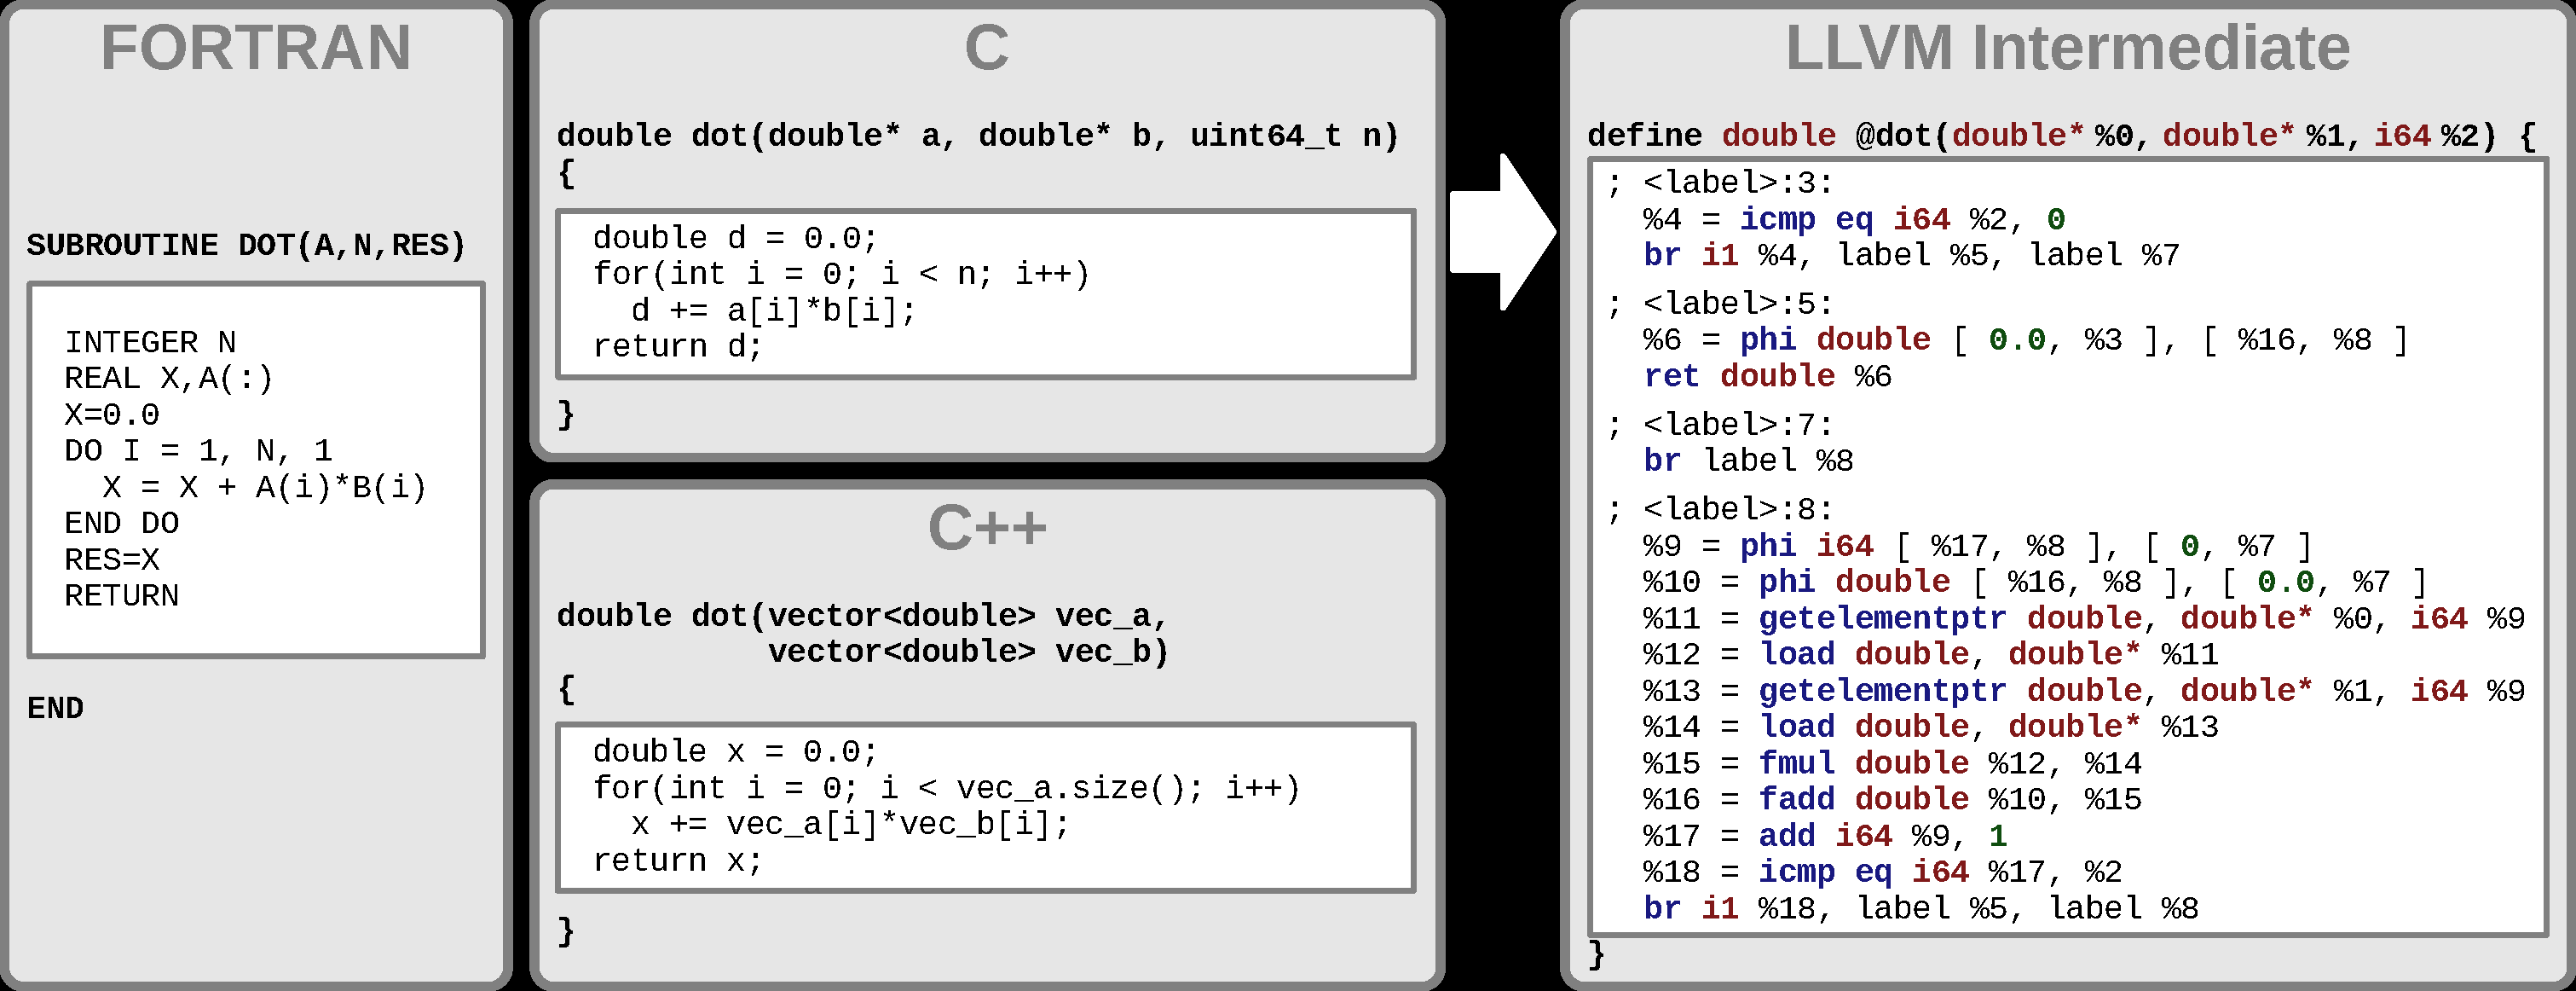
\includegraphics[width=\columnwidth]{figures/model_representations_textual}
\end{blackbox}

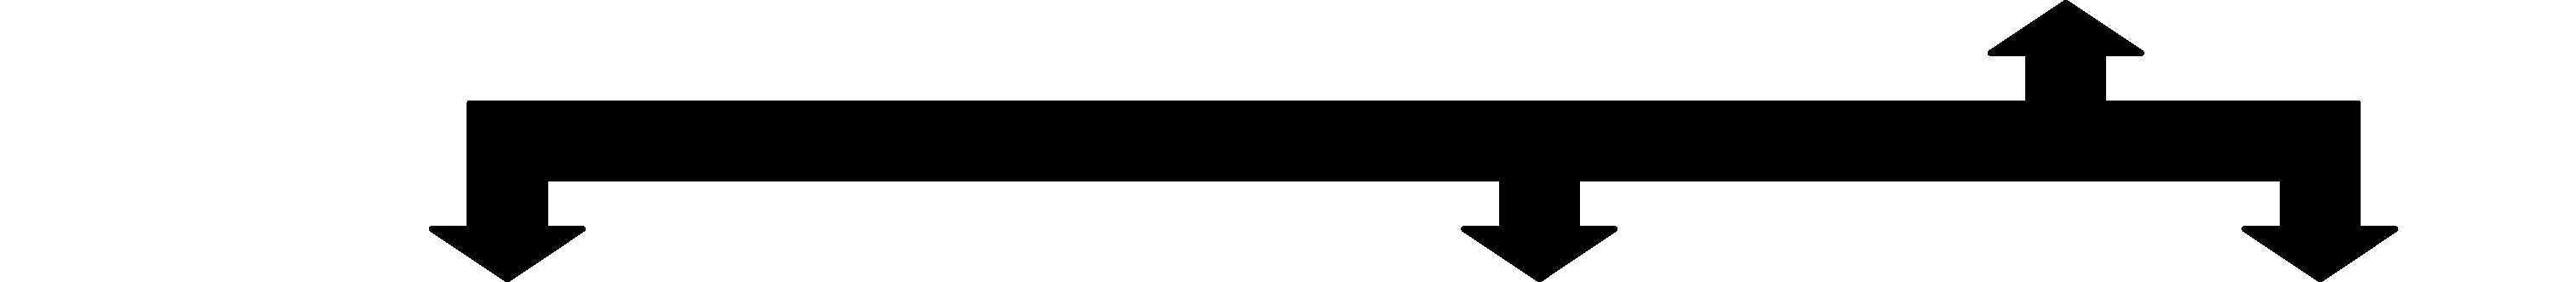
\includegraphics[width=\columnwidth]{figures/model_arrows_upper}

\begin{blackbox}{Data Structure Representation}
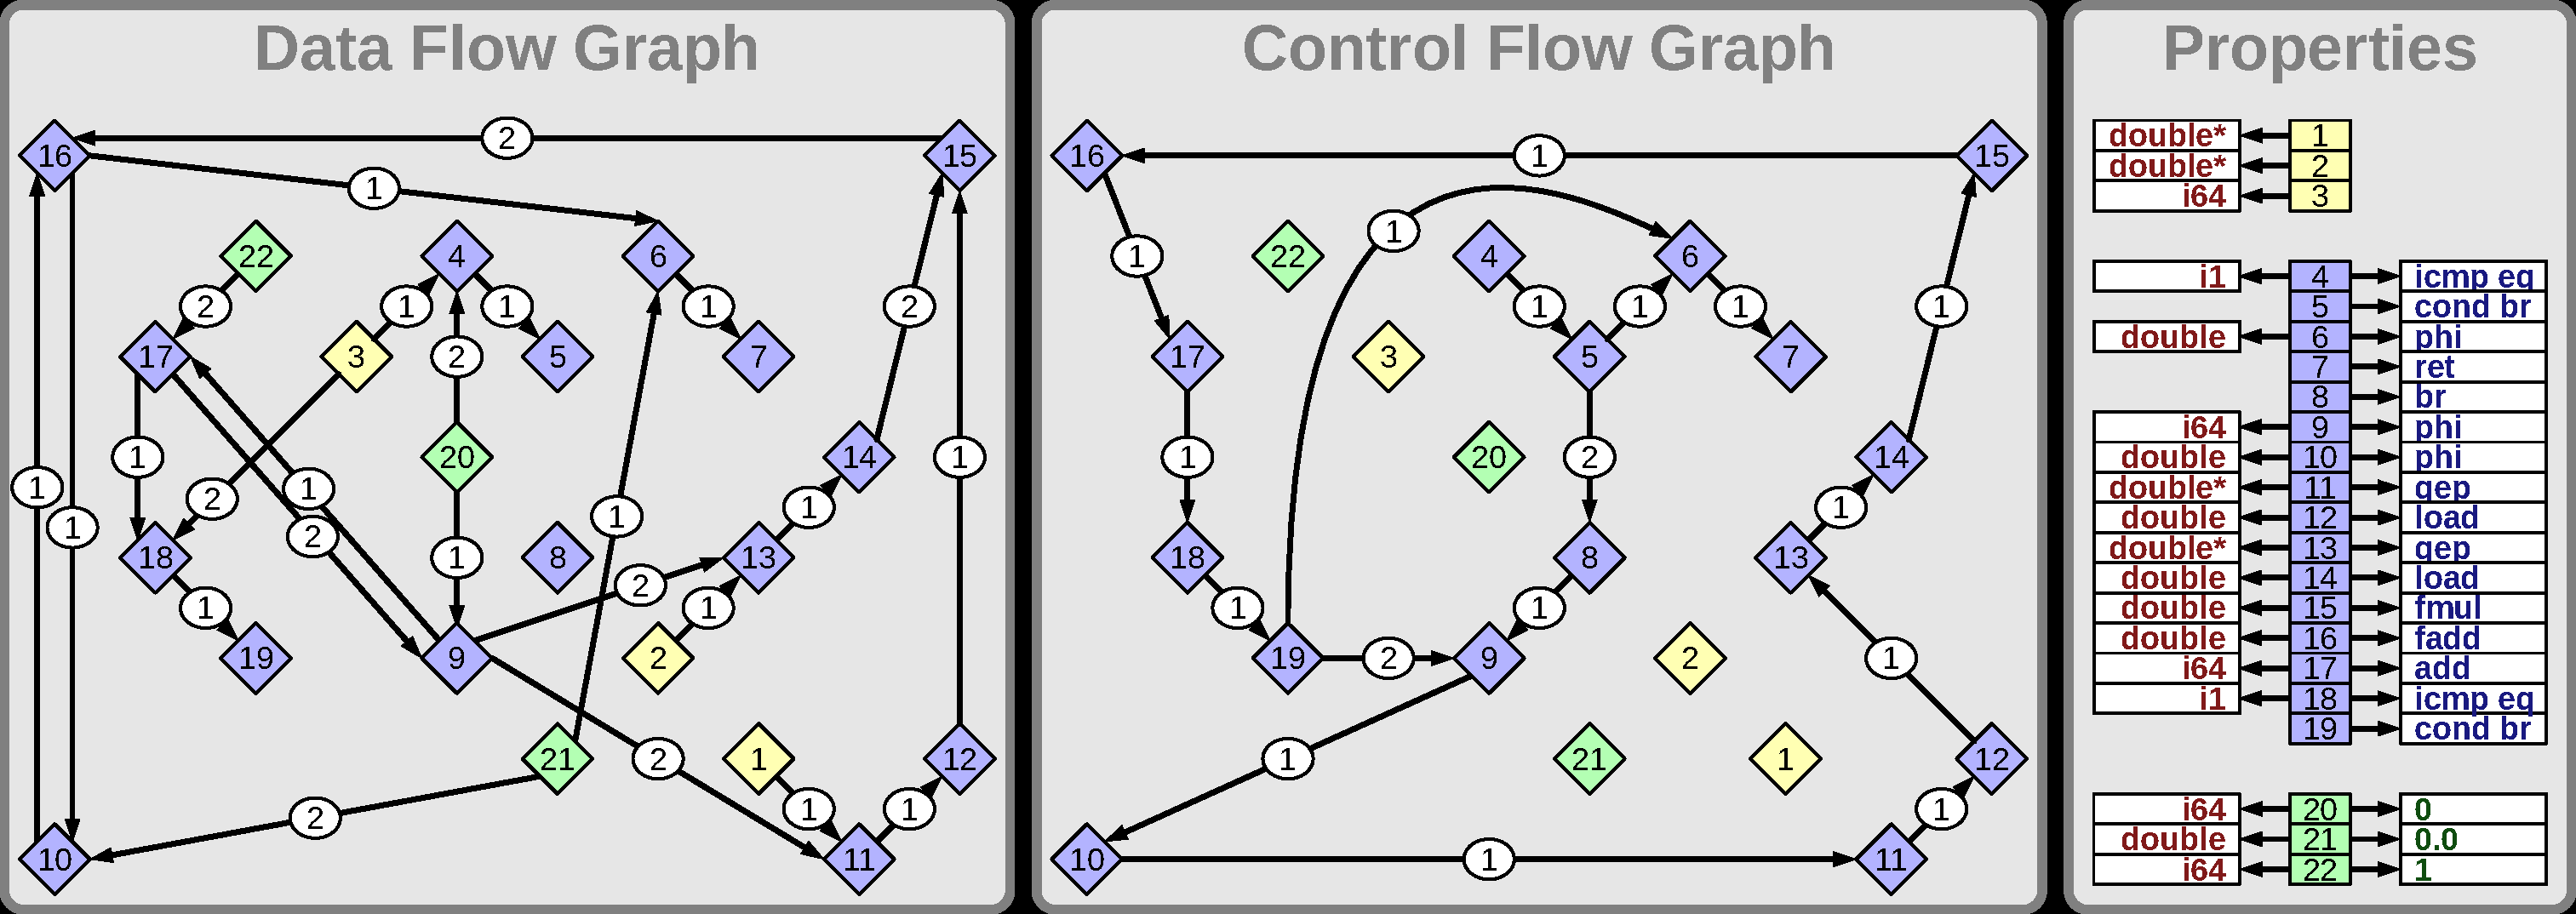
\includegraphics[width=\columnwidth]{figures/model_representations_structure}
\end{blackbox}

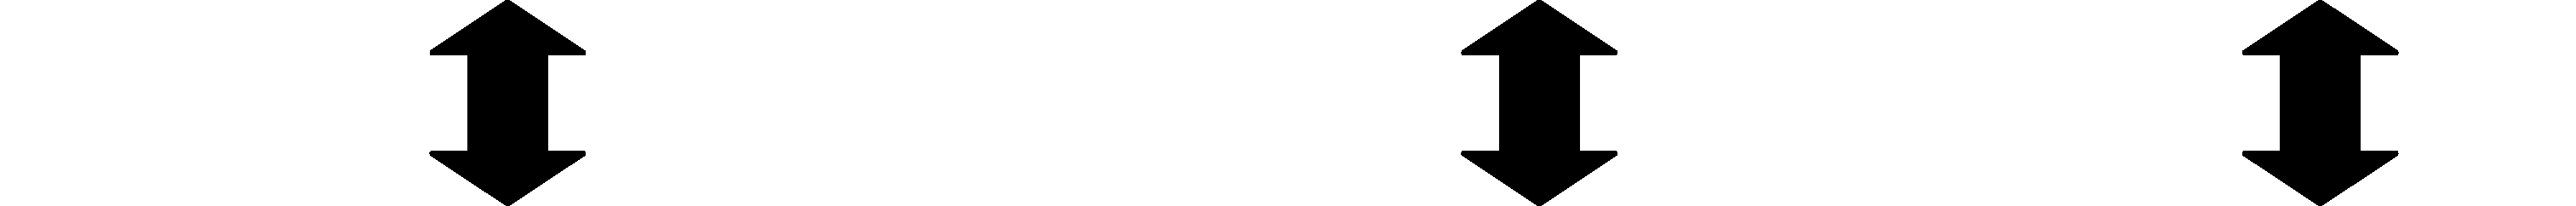
\includegraphics[width=\columnwidth]{figures/model_arrows_lower}

\begin{blackbox}{Mathematical Representation}
    \centering
    \begin{minipage}{0.329\textwidth}
        \begin{graybox}
            \scriptsize
            \setlength{\abovedisplayskip}{0pt}
            \setlength{\belowdisplayskip}{0pt}
            \vspace{-0.5em}
            \begin{align*}
                DF&G_\mathcal F=\{(1,11,1),(2,13,1)\\[-0.5em]
                  &(3,4,1),(3,18,2),(4,5,1),\\[-0.5em]
                  &(6,7,1),(9,11,2),(9,13,2),\\[-0.5em]
                  &(9,17,1),(10,16,1),(11,12,1),\\[-0.5em]
                  &(12,15,1),(13,14,1),(14,15,2),\\[-0.5em]
                  &(15,16,2),(16,6,1),(16,10,1),\\[-0.5em]
                  &(17,9,2),(17,18,1),(18,19,1),\\[-0.5em]
                  &(20,4,2),(20,9,1),(21,6,1),\\[-0.5em]
                  &(21,10,2),(22,17,2)\}\subset\mathbb N^3
            \end{align*}
        \end{graybox}
    \end{minipage}
    \begin{minipage}{0.329\textwidth}
        \begin{graybox}
            \scriptsize
            \setlength{\abovedisplayskip}{0pt}
            \setlength{\belowdisplayskip}{0pt}
            \vspace{-0.5em}
            \begin{align*}
                CFG_\mathcal F=\{&(4,5,1),(5,6,1),\\[-0.5em]
                  &(5,8,2),(6,7,1),\\[-0.5em]
                  &(8,9,1),(9,10,1),\\[-0.5em]
                  &(10,11,1),(11,12,1),\\[-0.5em]
                  &(12,13,1),(13,14,1),\\[-0.5em]
                  &(14,15,1),(15,16,1),\\[-0.5em]
                  &(16,17,1),(17,18,1),\\[-0.5em]
                  &(18,19,1),(19,6,1),\\[-0.5em]
                  &(19,9,2)\}\subset\mathbb N^3
            \end{align*}
        \end{graybox}
    \end{minipage}
    \begin{minipage}{0.329\textwidth}
        \centering
        \begin{graybox}
            \scriptsize
            \setlength{\abovedisplayskip}{0pt}
            \setlength{\belowdisplayskip}{0pt}
            \vspace{-0.5em}
            \begin{align*}
                T_\mathcal F={}&\{(1,\textit{double*}),(2,\textit{double*}),\dots\}\\[-0.5em]
                      \subset{}&\mathbb N\times Types_\text{LLVM}\\[-0.25em]
                P_\mathcal F={}&\{1,2,3\}\subset\mathbb N\\[-0.25em]
                I_\mathcal F={}&\{(4,\textit{icmp eq}),(5,\textit{cond br}),\dots\}\\[-0.5em]
                      \subset{}&\mathbb N\times Opcodes_\text{LLVM}\\[-0.25em]
                G_\mathcal F={}&\{\}\subset\mathbb N\\[-0.25em]
                C_\mathcal F={}&\{(20,0),(21,0),(22,1)\}\\[-0.5em]
                      \subset{}&\mathbb N\times\mathbb R
            \end{align*}

            \vspace{0.45em}
        \end{graybox}
    \end{minipage}

    \begin{minipage}{0.55\textwidth}
        \begin{graybox}
            \setlength{\abovedisplayskip}{0pt}
            \setlength{\belowdisplayskip}{0pt}
            \vspace{-0.5em}
            \begin{align*}
                M_{dot}=(DFG_\mathcal{F},
                 CFG_\mathcal{F},
                 T_\mathcal{F},
                 P_\mathcal{F},
                 I_\mathcal{F},
                 G_\mathcal{F},
                 C_\mathcal{F})
            \end{align*}
        \end{graybox}
    \end{minipage}
\end{blackbox}
\caption{Compiler-generated LLVM IR code is decomposed into data flow, control
         flow and per-value attributes.
         Mathematical notations of the three components are shown at the
         bottom.}
\label{fig:derivemaths}
\end{figure}

\section{Constraint Programming on SSA Programs}

    With a mathematical model of SSA programs in place, properties of such
    programs can now be formulated as constraint problems.
    For this purpose, \autoref{not:modelrepresentations} is introduced first,
    followed by the actual definition of {\em SSA constraint problem}s in
    \autoref{def:cprob}.

\begin{figure}[H]
\begin{notation}{Set of SSA Models}{modelrepresentations}
    Given a specific SSA representation (LLVM, Hydrogen, MIR, $\dots$), then
    denote $F$ the set of all valid functions that can be expressed in it.

    The {\em set of SSA models} $\mathcal M$ is defined as
    \begin{align*}
        \mathcal M := \{M\mid\exists\mathcal F\in F\colon M
                        \text{ is the SSA Model of }\mathcal F\}
    \end{align*}
\end{notation}

\begin{definition}{SSA constraint problem}{cprob}
    An SSA constraint problem $(V,C)$ is made up of a finite set of variables
    $V$ and a boolean predicate
    $C\colon\mathcal M\times\mathbb N^V\mapsto\{1,0\}$.
    The set of {\em constraint solutions} for a given constraint problem and a
    specific SSA model $M\in\mathcal M$ is given as
    \begin{align*}
        S_M(V,C) = \{s\in\mathbb N^V\mid C(M,s)=1\}.
    \end{align*}
\end{definition}
\end{figure}

    Some intuition is required here.
    The predicate function $C$ takes two arguments, firstly a tuple of integers
    and secondly a model of a function.
    The finite set $V$ identifies the elements withing the tuples, it can be
    thought of as a set of labels.
    The tuples of integers in $\mathbb N^V$ correspond to tuples of values
    within the function.
    The predicate function determines whether these values stand in a specific
    relationship to each other.
    Finally, the set of constraint solutions lists all those tuples, for which
    the predicate holds.

    The two parameters of $C$ -- integer tuple and model -- should be
    interpreted as two very different beasts here.
    The predicate evaluates whether a condition holds for the tuple of integers,
    the model on the other hand serves as the context for this evaluation.
    This is reflected in the definition of the set of constraint solutions,
    which is the set of all {\em true} evaluations given a fixed model.
    More pointedly, it makes sense to query ``all loops in a given function'',
    yet to ask for ``all functions with a specific loop'' is meaningless.

    The interesting aspect of this defition is now the structure of predicates
    $C$.
    This section will concern it self with how meaningful predicates can be
    composed from small building blocks and how the internal structure of the
    predicate can lead to efficient solver approaches.
    In order to evoke an intuition about these challenges, there will first be
    an example.

\subsection{Constraint Program Example}

\begin{figure}[p]
    
\raggedright
{\bf(a)} {} Initial problem statement:\\[1em]

\centering
{\LARGE$\underbrace{\text{Detect\vphantom{p}}}
                  _{\text{solver }S}
      \ \underbrace{\text{simple loop iterators}}
                  _{\text{SSA constraint problem }(V,C)}
                  \ \text{in the}
      \ \underbrace{\text{dot product function}}
                  _{\text{SSA model }M_{dot}}
                    \text{.}$}\\[2em]

\raggedright
{\bf(b)} {} Formulation as constraint problem:\\[1em]

\centering
\fontsize{60}{0}$S{}$\fontsize{20}{0}$\left(
\begin{minipage}{0.8\textwidth}
    \normalsize
    \begin{blackwhitebox}{\Large SSA constraint problem}
        \setlength{\abovedisplayskip}{0pt}
        \setlength{\belowdisplayskip}{0pt}
        \vspace{-0.5em}
        \begin{align*}
            V={}&\{\text{phi}, \text{update}, \text{step}\}\\
            C(M,x)={}&    ((1,x_\text{step})
                            \in C_\mathcal{F}\mathrel\land
                           (add,x_\text{update})
                            \in I_\mathcal{F}\mathrel\land\\
               &\phantom{(}(x_\text{phi},x_\text{update})
                            \in DFG_\mathcal{F}^*\mathrel\land
                           (x_\text{step},x_\text{update})
                            \in DFG_\mathcal{F}^*\mathrel\land\\
               &\phantom{(}(x_\text{update},x_\text{phi})
                            \in DFG_\mathcal{F}^*\mathrel\land
                           (phi,x_\text{phi})
                            \in I_\mathcal{F})
        \end{align*}
    \end{blackwhitebox}
    \begin{blackwhitebox}{\Large SSA model}
        \setlength{\abovedisplayskip}{0pt}
        \setlength{\belowdisplayskip}{0pt}
        \vspace{-0.5em}
        \begin{align*}
            DF&G_\mathcal F=\{(1,1,11),(1,2,13),(1,3,4),(2,3,18),(1,4,5),(1,6,7),\\[-0.5em]
              &(2,9,11),(2,9,13),\underline{(1,9,17)},(1,10,16),(1,11,12),(1,12,15),\\[-0.5em]
              &(1,13,14),(2,14,15),(2,15,16),(2,16,6),(2,16,10),\underline{(2,17,9)},\\[-0.5em]
              &(1,17,18),(1,18,19),(2,20,4),(1,20,9),(1,21,6),(1,21,10),\\[-0.5em]
              &\underline{(2,22,17)}\}\\[-0.25em]
            CF&G_\mathcal F=\{(1,4,5),(1,5,6),(2,5,8),(1,6,7),(1,8,9),(1,9,10),\\[-0.5em]
              &(1,10,11),(1,11,12),(1,12,13),(1,13,14),(1,14,15),\\[-0.5em]
              &(1,15,16),(1,16,17),(1,17,18),(1,18,19),(1,19,6),(2,19,9)\}\\[-0.25em]
            T_\mathcal F&{}=\{(\textit{double*},1),(\textit{double*},2),\dots\}\\[-0.25em]
            P_\mathcal F&{}=\{1,2,3\}\\[-0.25em]
            I_\mathcal F&{}=\{(\textit{icmp eq},4),(\textit{cond br},5),(\textit{phi},6),(\textit{ret},7),(\textit{br},8),\underline{(\textit{phi},9)},\\[-0.5em]
                        &(\textit{phi},10),(\textit{gep},11),(\textit{load},12),(\textit{gep},13),(\textit{load},14),(\textit{fmul},15),\\[-0.5em]
                        &(\textit{fadd},16),\underline{(\textit{add},17)},(\textit{icmp eq},18),(\textit{cond br},19)\}\\[-0.25em]
            G_\mathcal F&{}=\{\}\\[-0.25em]
            C_\mathcal F&{}=\{(0,20),(0,21),\underline{(1,22)}\}
        \end{align*}
    \end{blackwhitebox}
\end{minipage}
\right)$\\[2em]

\raggedright
\normalsize
{\bf(c)} {} Resulting set of constraint solutions:\\[1em]

\centering
{\LARGE$S_{M_{dot}}(V,C)=\{\{\text{phi}\mapsto9,
                             \text{update}\mapsto17,
                             \text{step}\mapsto22\}\}\subset\mathbb N^V$}
\caption{Detection of simple loop iterators is formulated as a constraint
         problem and applied to the SSA model from \autoref{fig:derivemaths}.
         One solution corresponding to the source variable {\tt i} is found.}
\label{fig:constraintsolution}
\end{figure}

    Consider the task of detecting in a program all simple loop iterator in a
    function, shown in \autoref{fig:constraintsolution}.
    The top {\bf a)} demonstrates how this can be translated into a constraint
    problem, solved in the context of an SSA model.
    For demonstration purposes, the SSA model that was derived in
    \autoref{fig:derivemaths} is used.

    Simple loop iterators show up in LLVM IR as data flow cycles with a phi node
    and an add instruction.
    This is expressed as a constraint problem at the top of the second part
    {\bf b)} of the figure.
    The formulation introduces the variables
    $V=\{\text{phi}, \text{update}, \text{step}\}$ and a predicate to
    describe the required conditions on the variables.
    The predicate is decomposed with logical conjunctions (``$\land$'') into
    several {\em elemt-of} relationships that have to hold simultaneously on the
    structures of the model.
    Explicit control flow constraints for establishing the loop strucure are not
    required, as the data flow with the $\Phi$ node already implies the presence
    of a loop structure.
    Below the predicate formulation is the SSA model from
    \autoref{fig:derivemaths}.

    At the bottom {\bf c)} of the figure, the set of constraint solutions is
    shown.
    It contains as its only element the tuple
    $\{\text{phi}\mapsto6,\text{update}\mapsto14,\text{step}\mapsto19\}$.
    Note that elements of $\mathbb N^V$ can be identified as mappings
    $V\rightarrow\mathbb N$.
    The underlined strucures in the lower part of
    \autoref{fig:constraintsolution} {\bf b)} demonstrate the validity of the
    solution:
    $(22,1)\in C_\mathcal F$ and $(9,17,1)\in DFG_\mathcal F$ and
    $(22,17,2)\in DFG_\mathcal F$ and $(9,\textit{phi})\in I_\mathcal F$ and
    $(17,\textit{add})\in I_\mathcal F$ and $(17,9,2)\in DFG_\mathcal F$,
    corresponding to the six simple constraints that make up the predicate.

    Each solution therefore assigns an integer to each variable.
    With the help of \autoref{fig:derivemaths}, the specific values $9,17,22$
    can be identified with lines 14 and 17, as well as the constant 1 in the
    LLVM IR code from \autoref{llvmirexample} {\bf b)}.
    This corresponds to the loop iterator \texttt{i} in the C source code of the
    \texttt{dot} function, correctly identifying the only simple loop iterator.

    With a detailed derivation of the SSA model completed and some intuition
    about the nature of constraint problems, only the solver $S$ in
    \autoref{fig:constraintsolution} remains a black box.
    The next sections derive how a backtracking solver can
    be used to efficiently compute the set of solutions.

\subsection{Solving of SSA Constraint Problems}

    A solver for SSA constraint problems needs to efficiently compute $S_M(V,C)$
    for some concrete $(V,C)$ and $M$.
    This is a search problem:
    All values in $\mathbb N^V$ that satisfy $C$ with the context $M$ need to
    be identified.
    $\mathbb N^V$ is infinitely large, so this requires non-trivial
    computational approaches, even when the direct evaluation of $C$ for any
    potential solution can be performed efficiently.
    However, backtracking can be used to find partial solutions, which are
    incrementally extended.
    This effectively prunes the search space.

\begin{figure}[h]
    \begin{definition}{Backtracking Solution of Constraint Problems}{backtracking}
        Given a constraint problem $(V,C)$, an order $V=\{v_1,\dots,v_n\}$ can
        be choosen.

        Then a collection $(P_k)_{k=1\dots n}$ of boolean predicates
        $P_k:\mathcal M\times \mathbb N^{k-1}\times\mathbb N\rightarrow\{0,1\}$
        is a {\em backtracking solution} of $(V,C)$ if and only if the
        following is satisfied or all $x\in\mathbb N^V$:
        \begin{align}
            C(M,x)=1\iff P_k(M,(x_{v_l})_{l=1\dots k-1},x_{v_k})=1\text{ for all }1\leq k\leq n.
        \end{align}
    \end{definition}
\end{figure}

    Using \autoref{def:backtracking}, the backtracking search shown in
    \autoref{backtrackalg} can be implemented.
    The variable $x$ iterates over $\mathbb N^n$
    (which is identified with $\mathbb N^V$ in line 7), while the variable $k$
    tracks the number of currently considered dimensions of this partial
    solution.
    After initialisation in line 2, a single loop spans the remainder of the
    algorithm.
    In each iteration, the algorithm tries to assign a valid value to the latest
    element in the partial solution in line 4.
    If this fails, the algorithm backtracks in lines 12--17.
    Otherwise, the solution is either complete (lines 6--8), or the algorithm
    increases the size of the partial solution in lines 9--11 and continues the
    search for the next element of $x$ in the following iteration.

\begin{algorithm}[H]
    \caption{Basic backtracking algorithm}
    \begin{algorithmic}[1]
        \Procedure{Detect}{$M,(P_k)_{k=1\dots n}$}\vspace{-0.45em}
            \State $k\gets1$,\quad$x\gets(1,\dots,1)\in\mathbb N^n$\vspace{-0.45em}
            \While{$true$}\vspace{-0.45em}
                \State $x_k\gets min\{y\in\mathbb N\mid y\geq x_k\mathrel\land P_k(\{x_1,\dots,x_{k-1},y\},M)=1\}$\vspace{-0.45em}
                \If{$x_k<\infty$}\vspace{-0.45em}
                    \If{$k=n$}\vspace{-0.45em}
                        \State {\bf yield} $\{v_k\mapsto x_k\}_{k=1\dots n}\in\mathbb N^V$\vspace{-0.45em}
                        \State $x_k\gets x_k+1$\vspace{-0.45em}
                    \Else\vspace{-0.45em}
                        \State $k\gets k+1$\vspace{-0.45em}
                        \State $x_k\gets1$\vspace{-0.45em}
                    \EndIf
                \Else\vspace{-0.45em}
                    \State $k\gets k-1$\vspace{-0.45em}
                    \If{$k\geq1$}\vspace{-0.45em}
                        \State$x_k\gets x_k+1$\vspace{-0.45em}
                    \Else\vspace{-0.45em}
                        \State {\bf exit}
                    \EndIf
                \EndIf
            \EndWhile
        \EndProcedure
    \end{algorithmic}
    \label{backtrackalg}
\end{algorithm}

    
    In order to implement this algorithm, the set in line $4$ has to be
    available in each iteration.
    Even when assuming that the direct evaluation of $C$ is possible in an
    efficient manner, this is not obviously true.
    Fortunately, there is a large class of useful SSA constraint problems, for
    which this set can be efficiently computed.

\subsection{Structure of Basic SSA Constraint Problems}

    The most basic construction rules for SSA constraint problems are the
    element-of constraint problem introduced in \autoref{def:elementofconstr}
    and the conjunction and disjunction constraint problems in
    \autoref{def:conjconstr}.
    These already allow the formulation of interesting SSA constraint problems
    in their own, as previously seen in \autoref{fig:constraintsolution}.
    Implicitly, this requires the definition of constraint problems on a
    larger set of variables, as introduced in \autoref{def:constrext}.

\begin{figure}[h]
    \begin{definition}{Element-of Constraint Problem}{elementofconstr}
        For a set of tuples $S(M)\subset\mathbb N^V$ that is potentially
        dependent on the SSA model $M\in\mathcal M$
        (i.e.\ $S(M):=DFG_\mathcal F^*$),
        the element-of constraint problem $(V,E_S)$ is given by
        \begin{align*}
            E_S(M,x)=\left\{\begin{array}{l}
                                1\text{\quad if }x \in S(M)\\
                                0\text{\quad otherwise}.
                            \end{array}\right.
        \end{align*}
    \end{definition}

    \begin{definition}{Conjunction and Disjunction Constraint}{conjconstr}
        For two constraint problems $(V,C)$ and $(V,C')$, the
        conjunction constraint $(V,C\mathrel\land C')$ and the
        disjunction constraint $(V,C\mathrel\lor C')$ are given by
        \begin{align*}
            &C\mathrel\land C'(M,x):=\left\{
                \begin{array}{l}
                    1\text{\quad if }C(M,x)=1\mathrel\land C'(M,x)=1\\
                    0\text{\quad otherwise}
                \end{array}\right.\\
            &C\mathrel\lor C'(M,x):=\left\{
                \begin{array}{l}
                    1\text{\quad if }C(M,x)=1\mathrel\lor C'(M,x)=1\\
                    0\text{\quad otherwise}.
                \end{array}\right.
        \end{align*}
    \end{definition}

    \begin{definition}{Extension of Constraint Problems}{constrext}
        For an SSA constraint problem $(V,C)$ and an injection
        $i:V\hookrightarrow W$, the constraint problem $(W,C^W)$ is given by
        \begin{align*}
            C^W(M,x):=C(M,\{x_{i(v)}\}_{v\in V}).
        \end{align*}
    \end{definition}
\end{figure}

    For SSA constraint problems that are constructed according to these rules,
    backtracking solutions can be directly constructed as shown in
    \autoref{theo:theo1}, \autoref{theo:theo2}, \autoref{theo:theo3} and
    \autoref{theo:theo4}.
    Note that this appears mostly tautological at first, but there are some
    pitfalls.
    For the disjunction rule, the backtracking solution is not the obvious one.

\begin{figure}[p]
    \begin{theorem}{Backtracking Solution for Element-of Constraint Problems}{theo1}
        For $S\subset\mathbb N^V$, the predicates $(P_k[E_S])_{k=1\dots n}$
        defined by
        \begin{align*}
            P_k[E_S](M,x,y):=\left\{
                \begin{array}{ll}
                    1&\text{if }y\in R_k(M,x)\\
                    0&\text{otherwise},
                \end{array}\right.
        \end{align*}
        give a backtracking solution of $(V,E_S)$, where $R_k(M,x)$ is given by
        \begin{align*}
            R_k(M,x)=\{s_{v_k}\mid s\in S(M),s_{v_1}=x_1,\dots,s_{v_{k-1}}=x_{k-1}\}.
        \end{align*}
        \tcblower
        \paragraph*{Proof:} The definition of $E_S$ gives 
        \begin{align*}
            E_S(M,x)=1\iff x\in S(M).
        \end{align*}
        Directly from the definition of $R_k$ then follows
        \begin{align*}
            x\in S(M)\iff x_{v_k}\in R_k(M,\{x_{v_1},\dots,x_{v_{k-1}}\})\text{ for all }k.
        \end{align*}
        Therefore, the equivalence from \autoref{def:backtracking} holds.
    \end{theorem}
    \begin{theorem}{Backtracking Solution for Conjunction Constraint problems}{theo2}
        For SSA constraint problems $(V,C)$ and $(V,C')$ with backtracking
        solutions $(P_k)_{k=1\dots n}$ and $(P'_k)_{k=1\dots n}$, the
        predicates $(P_k[C\mathrel\land C'])_{k=1\dots n}$ defined by
        \begin{align*}
            P_k[C\mathrel\land C'](M,x,y):=\left\{
                \begin{array}{ll}
                    1&\text{if }P_k(M,x,y)=1\mathrel\land P'_k(M,x,y)=1\\
                    0&\text{otherwise},
                \end{array}\right.
        \end{align*}
        give a backtracking solution of $(V,C\mathrel\land C')$.
        \tcblower
        \paragraph*{Proof:}
        The definition of $(V,C\mathrel\land C')$ together with the
        assumption that \autoref{def:backtracking} holds for the two given
        backtracking solutions gives
        \begin{align*}
            C\mathrel\land C'(M,x)=1\iff{}& P_k(M,(x_{v_1},\dots,x_{v_{k-1}}),x_{v_k})=1\text{ for all }k\\
                                  \mathrel\land{}& P'_k(M,(x_{v_1},\dots,x_{v_{k-1}}),x_{v_k})=1\text{ for all }k.
        \end{align*}
        With the definition of $P_k[C\mathrel\land C']$, this immediately gives
        \begin{align*}
            C\mathrel\land C'(M,x)=1\iff P_k[C\mathrel\land C']&(M,(x_{v_1},\dots,x_{v_{k-1}}),x_{v_k})\text{ for all }k.
        \end{align*}
        Therefore, the equivalence from \autoref{def:backtracking} holds.
    \end{theorem}
\end{figure}

\begin{figure}[p]
    \begin{theorem}{Backtracking Solution for Extensions of Constraint Problems}{theo3}
        For an SSA constraint problem $(V,C)$ with a backtracking
        solution $(P_k)_{k=1\dots n}$ and a set $W$ with an injection
        $i:V\hookrightarrow W$ and an order $W=\{w_1,\dots,w_n\}$ that is
        compatible with the order on $V$ in the sense that $v_k=w_{t(k)}$ with
        some $t:\mathbb N\rightarrow\mathbb N$ strictly increasing, the
        predicates $(P_k[C^W])_{k=1\dots |W|}$ defined by
        \begin{align*}
            P_k[C^W](M,x,y):=\left\{
                \begin{array}{ll}
                    P_k\left(M,\left(x_{t(1)},\dots,x_{t(n)}\right),y\right)&\text{if }w_k\in V\\
                    \equiv 1&\text{otherwise}\\
                \end{array}\right.
        \end{align*}
        give a backtracking solution of $(V,C^W)$.
        \tcblower
        \paragraph*{Proof:} trivial
    \end{theorem}
    \begin{theorem}{Backtracking Solution for Disjunction Constraint problems}{theo4}
        For SSA constraint problems $(V,C)$ and $(V,C')$ with backtracking
        solutions $(P_k)_{k=1\dots n}$ and $(P'_k)_{k=1\dots n}$, the
        predicates $(P_k[C\mathrel\lor C'])_{k=1\dots n}$ defined by
        \begin{align*}
            P_k[C\mathrel\lor C'](M,x,y):={}&\left(R_{k,1}(M,x,y)\mathrel\land P_k(M,x,y)\right)\\
                              \mathrel\lor{}&\left(R_{k,2}(M,x,y)\mathrel\land P'_k(M,x,y)\right)
        \end{align*}
        give a backtracking solution of $(V,C\mathrel\lor C')$, were $R_k(M,x)\in\{0,1\}^2$
        is given by 
        \begin{align*}
            R_0=\{1,1\}&&
            R_k(M,x)=\left(
                \begin{array}{l}
                    R_{k-1,1}(M,x)\mathrel\land P_k(M,(x_1,\dots,x_{k-2}),x_{k-1})\\
                    R_{k-1,2}(M,x)\mathrel\land P'_k(M,(x_1,\dots,x_{k-2}),x_{k-1})
                \end{array}\right)
        \end{align*}
        \tcblower
        \paragraph*{Proof:} The equivalence from \autoref{def:backtracking}
                            holds by assumption for the backtracking solutions
                            of $(V,C)$ and $(V,C')$, therefore
        \begin{align*}
            C\mathrel\lor C'(M,x)=1\iff{}& P_k(M,(x_{v_1},\dots,x_{v_{k-1}}),x_{v_k})=1\text{ for all }k\\
                                  \mathrel\lor{}& P'_k(M,(x_{v_1},\dots,x_{v_{k-1}}),x_{v_k})=1\text{ for all }k
        \end{align*}
        By definition of $P_k[C\mathrel\lor C']$ this gives
        \begin{align*}
            C\mathrel\lor C'(M,x)=1\iff{}P_n[C\mathrel\lor C'](M,(x_{v_1},\dots,x_{v_{n-1}}),x_{v_n})=1.
        \end{align*}
        This is sufficient for the equivalence from \autoref{def:backtracking}
        in both directions, due to
        \begin{align*}
            P_n[C\mathrel\lor C'](M,x,y)\implies P_k[C\mathrel\lor C'](M,(x_1,\dots,x_{k-1}),x_k)\text{ for all }k.
        \end{align*}
    \end{theorem}
\end{figure}

\subsection{Backtracking Example}

\begin{figure}[p]
    \begin{blackwhitebox}{Original SSA constraint problem}
        \setlength{\abovedisplayskip}{0pt}
        \setlength{\belowdisplayskip}{0pt}
        \vspace{-0.5em}
        \begin{align*}
            V&{}=\{\text{phi}, \text{update}, \text{step}\}\\
            C(M,v)=         ({}&(v_\text{step},1)
                                 \in C_\mathcal{F}
                \mathrel\land   (v_\text{phi},v_\text{update})
                                 \in DFG_\mathcal{F}^*\\
                \mathrel\land{}&(v_\text{step},v_\text{update})
                                 \in DFG_\mathcal{F}^*
                \mathrel\land   (v_\text{phi}, phi)
                                 \in I_\mathcal{F}\\
                \mathrel\land{}&(v_\text{update}, add)
                                 \in I_\mathcal{F}
                \mathrel\land   (v_\text{update},v_\text{phi})
                                 \in DFG_\mathcal{F}^*)
        \end{align*}
    \end{blackwhitebox}
    \begin{blackwhitebox}{Backtracking Solution}
        \setlength{\abovedisplayskip}{0pt}
        \setlength{\belowdisplayskip}{0pt}
        \vspace{-0.5em}
        \begin{align*}
            v_1={}&\text{phi}\\
            P_1[C](M,y)=      (&1
                \mathrel\land   y\in\{s_1\mid s\in DFG_\mathcal{F}\}\\
                \mathrel\land{}&1
                \mathrel\land   y\in\{s_1\mid s\in I_\mathcal{F}, s_2=phi\}\\
                \mathrel\land{}&1
                \mathrel\land   y\in\{s_2\mid s\in DFG_\mathcal{F}\})\\[1em]
                       =      (&y\in\{s_1\mid s\in DFG_\mathcal{F}\}\\
                \mathrel\land{}&y\in\{s_1\mid s\in I_\mathcal{F}, s_2=phi\}\\
                \mathrel\land{}&y\in\{s_2\mid s\in DFG_\mathcal{F}\})\\[1em]
            v_2={}&\text{update}\\
            P_2[C](M,x,y)=    (&1
                \mathrel\land   y\in\{s_2\mid s\in DFG_\mathcal{F},s_1=x_1\}\\
                \mathrel\land{}&y\in\{s_2\mid s\in DFG_\mathcal{F}\}
                \mathrel\land   1\\
                \mathrel\land{}&y\in\{s_1\mid s\in I_\mathcal{F},s_2=add\}
                \mathrel\land   y\in\{s_2\mid s\in DFG_\mathcal{F},s_2=x_1\})\\[1em]
                         =    (&y\in\{s_2\mid s\in DFG_\mathcal{F},s_1=x_1\}\\
                \mathrel\land{}&y\in\{s_1\mid s\in I_\mathcal{F},s_2=add\}
                \mathrel\land   y\in\{s_2\mid s\in DFG_\mathcal{F},s_2=x_1\})\\[1em]
            v_3={}&\text{step}\\
            P_3[C](M,x,y)=  ({}&y\in\{x_1\mid x\in C_\mathcal{F}, x_2=1\}
                \mathrel\land   1\\
                \mathrel\land{}&y\in\{x_1\mid x\in DFG_\mathcal{F}, x_2=v_{update}\})
                \mathrel\land   1\\
                \mathrel\land{}&1
                \mathrel\land   1\\[1em]
                         =  ({}&y\in\{x_1\mid x\in C_\mathcal{F}, x_2=1\}\\
                \mathrel\land{}&y\in\{x_1\mid x\in DFG_\mathcal{F}, x_2=v_{update}\})
        \end{align*}
    \end{blackwhitebox}
\end{figure}

    With the theorems from the previous section, a backtracking solution can
    be found for the previous example, as shown on the right.

%
%\section{Implementation of Constraint Predicates}
%
%    With the solver approach derived, it now needs to be established how real
%    constarint problem predicates can be algorithmically implemented in order
%    to evaluate the required functions.
%
%\subsection{Important Graph Properties}
%
%    With our established notation, we can now transfer standard compiler
%    analysis problems into this more formal language.
%    Most of these are based on graph theoretic considerations, so we
%    will firstly need to recapitulate some graph theory basics.
%    Firstly, there is the notion of {\em cuts} of graphs, that we will introduce
%    here in a hybrid version of edge based and vertex based modelling.
%
%    \begin{definition}{Connections and Cuts}{def:cuts}
%        Consider an adjacency set $E\subset\mathbb{N}\times\mathbb{N}$ of a
%        directed graph and let $a,b\in\mathbb{N}$.
%        \newline
%        A {\em connection} between $a$ and $b$ in $E$ is a subset
%        $A\subset\mathbb{N}$ such that a finite sequence $c_1,\dots,c_n$
%        exists with
%        \begin{gather*}
%            a=c_1\hspace{1cm}c_2,\dots,c_{n-1}\in A\hspace{1cm}b=c_n\\
%            (c_k,c_{k+1})\in E\hspace{1em}\text{for all}\hspace{1em}k=1,\dots,n-1.
%        \end{gather*}
%        A {\em cut} between $a$ and $b$ in $E$ is a subset $B\subset E$
%        such that no {\em connection} between $a$ and $b$ in $E\setminus B$
%        exists.
%        We define the {\em set of cuts} between $a$ and $b$ in $E$ as
%        \begin{align*}
%            \text{Cuts}_E(a,b):=\{B\subset E\mid B\text{ is {\em cut} between $a$ and $b$ in $E$}\}
%        \end{align*}
%    \end{definition}
%
%    These notions are quite intuitive, two vertices in a graph have a connection
%    if one can reach the other via the available edges and by ``cutting'' these
%    edges, they are no longer connected.
%
%    These definitions are very useful in order to identify crucial properties of
%    data and control flow graphs.
%    Most standard is the the definition of a dominator in the control flow
%    graph: An instruction $d$ is said to dominate another instruction $n$ if
%    every path from the entry node to $n$ through the control flow graph must
%    go through $d$.
%    In our model this is of course equivalent to the following:
%
%    \begin{definition}{Dominator}{def:dominator}
%        Consider an instruction $n$ in a function $\mathcal F$.
%        A {\em dominator} of $n$ in $\mathcal{F}$ is an instruction $d$ such
%        that $\{(d,m)\mid(d,m)\in CFG_\mathcal{F}^*\}$ is a {\em cut} between $1$ and $n$ in $CFG_\mathcal{F}^*$.
%    \end{definition}
%
%    Another important definition is the concept of control dependence.
%    Control dependence models the behaviour of conditional control flow.
%    Instructions that are executed only in some control flow paths are control
%    dependent on the conditional branches that preceed them.
%
%    \begin{definition}{Control Dependence}{cdg}
%        Consider instructions $a,b$.
%        We say that an $b$ is control dependent on $a$ if a instructions
%        $c,c'$ exist such that $(a,c),(a,c')\in CFG_\mathcal{F}^*$ and
%        \begin{align*}
%            \{(a,c)\}\in{}&{}\text{Cuts}_E(a,b)\\
%            \{(a,c')\}\notin{}&{}\text{Cuts}_E(a,b)\text{.}
%        \end{align*}
%        We define the {\em control dependence graph} as follows
%        \begin{align*}
%            CDG_\mathcal{F}:=\{(a,b)\in\mathbb{N}^2\mid b\text{ control dependent on }a\}
%        \end{align*}
%    \end{definition}
%
%\begin{figure}[p]
%    \centering
%    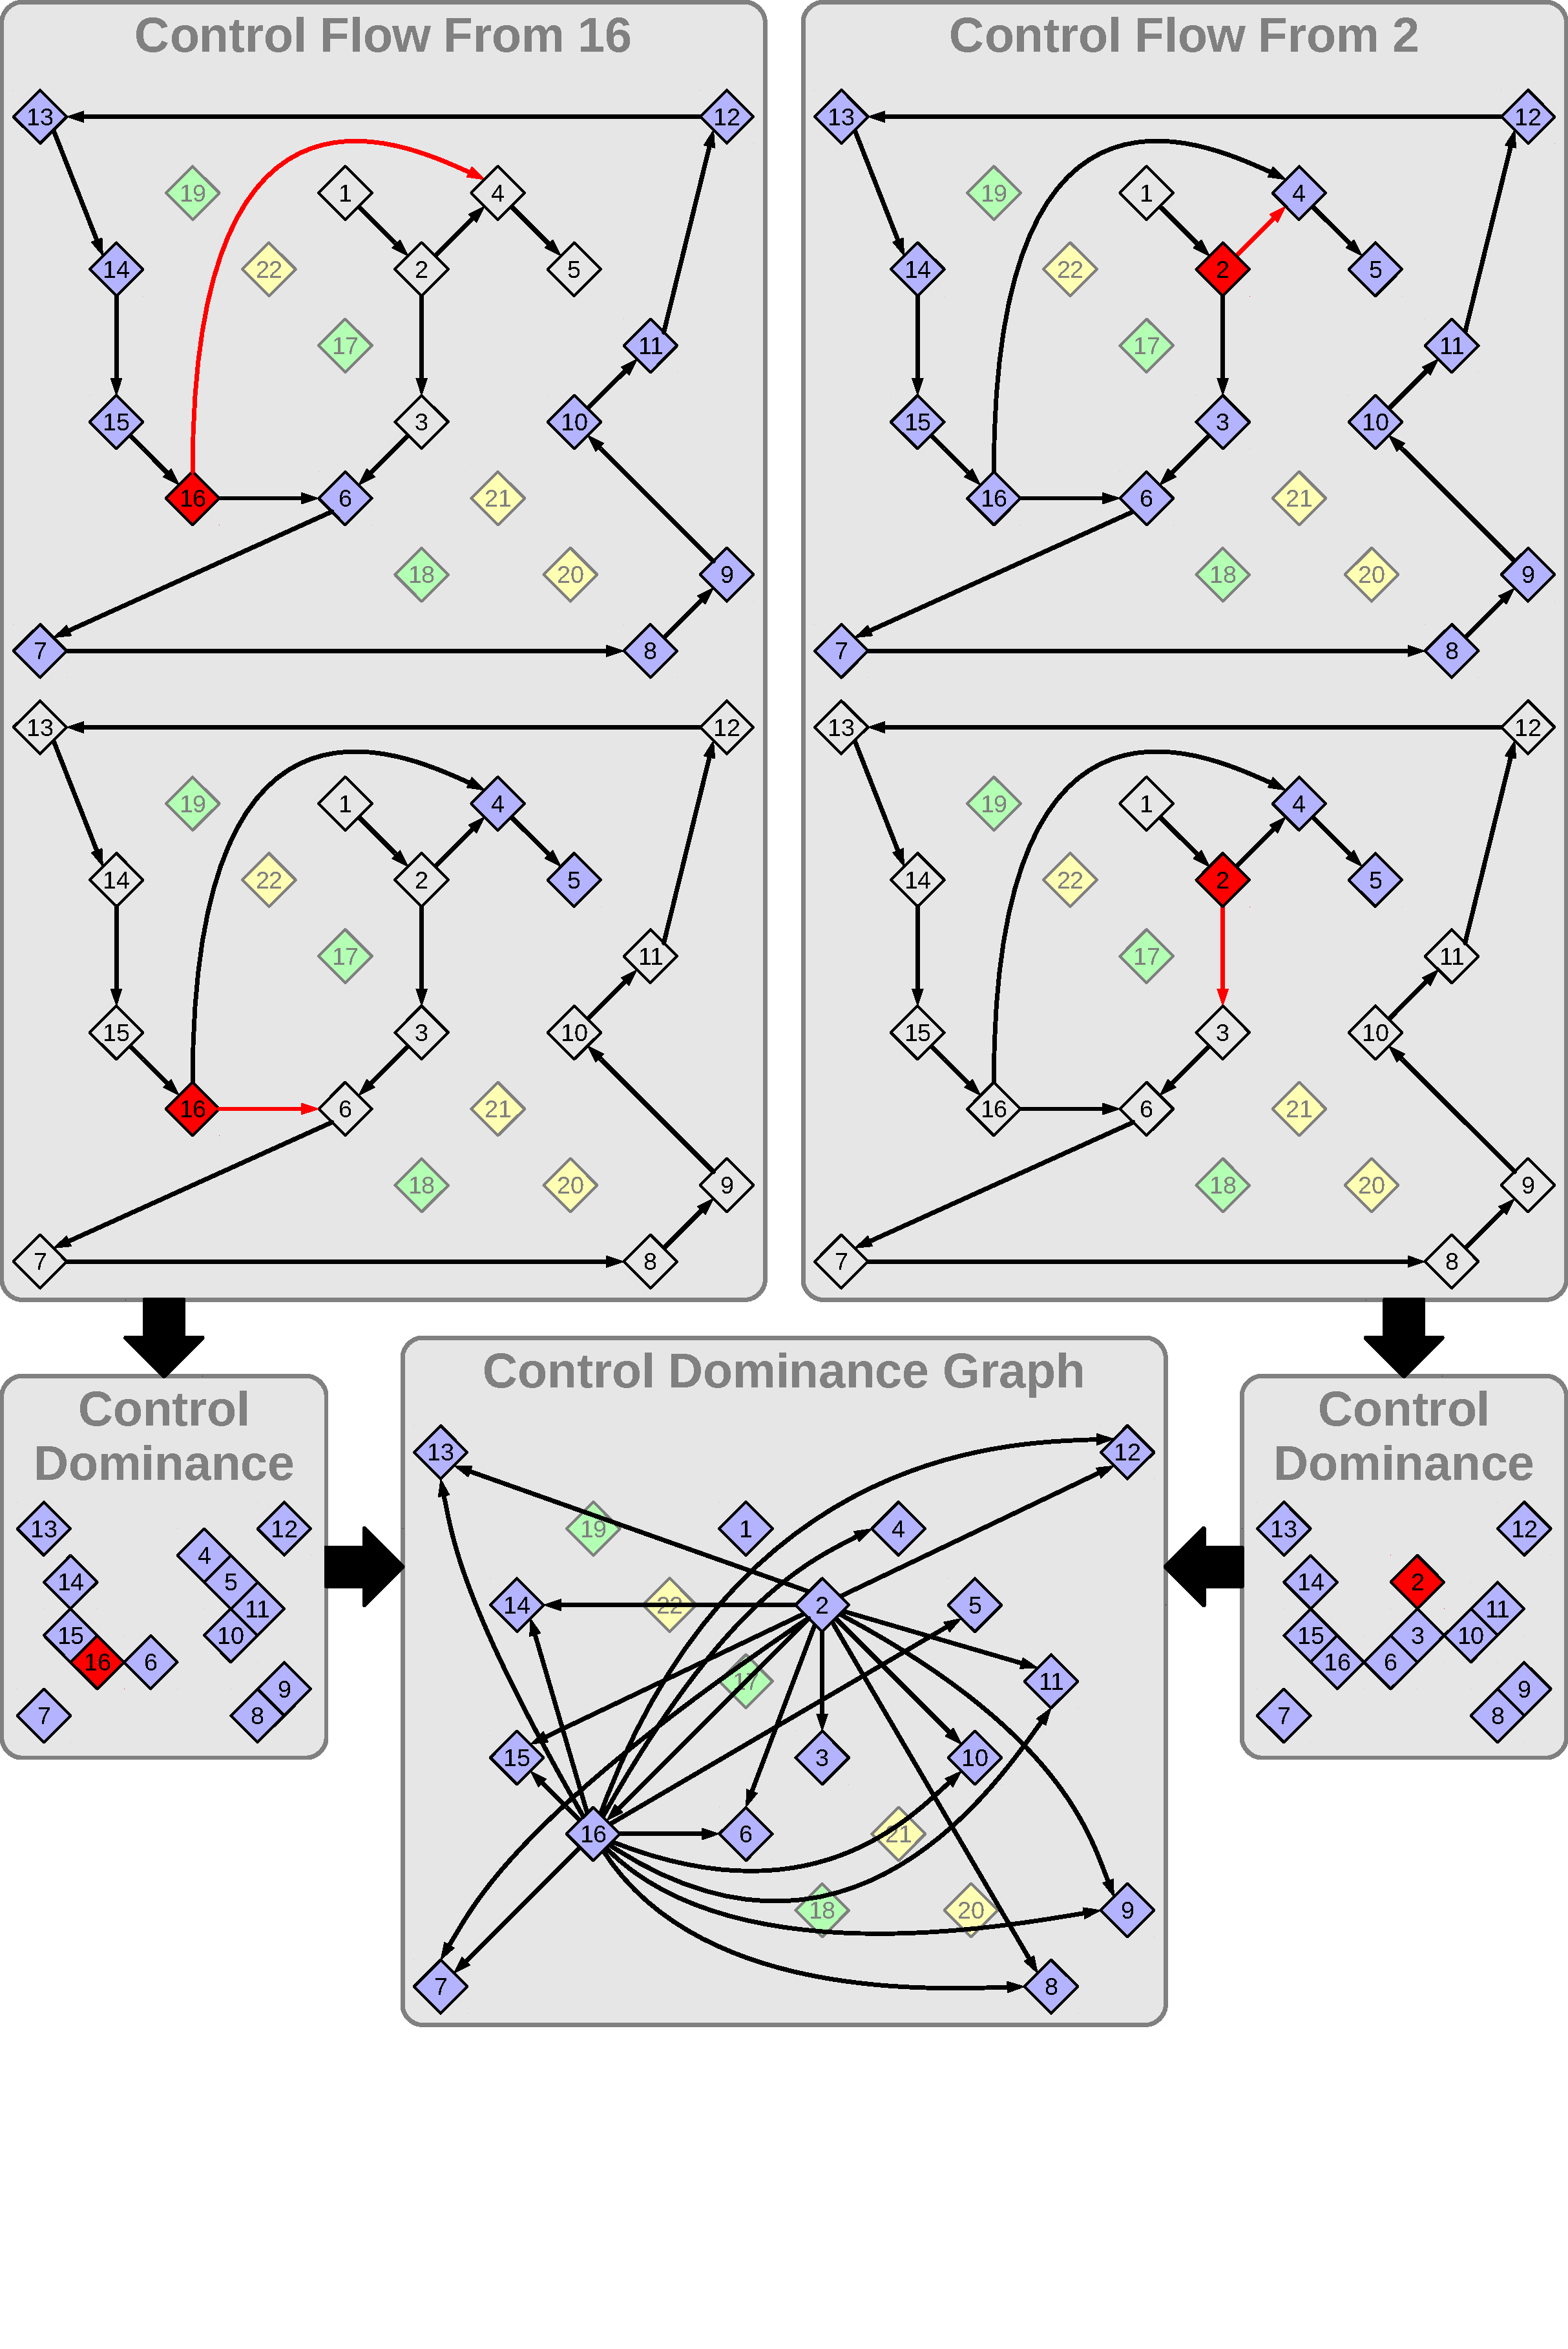
\includegraphics[width=\textwidth,height=1.5\textwidth]{figures/schaubild2.pdf}
%
%    \vspace{27.38136pt}
%    \caption{Computation of the control dependence graph.}
%    \label{fig:pdg}
%\end{figure}
%
%\subsection{Control Dependence Example}
%
%    The control dependence graph is a function of the control flow graph, as is
%    directly apparent from \autoref{def:cdg}.
%    We can see how an example control dependence graph is computed in
%    \autoref{fig:pdg}, from the control flow graph of the \texttt{dot} function
%    in \autoref{fig:derivemaths}.
%    From the definition it is immediately obvious that we need to only consider
%    conditional branches as origins of control dependence.
%
%    We can consider the two conditional branches $2$ and $16$ independently.
%    On the right, we consider only $2$.
%    We check the defining property: On the top of the figure, all the
%    instructions that are not reachable from $2$ without the edge $(2,4)$ are in
%    grey.
%    Below this, all instructions not reachable from $2$ without $(2,3)$ are
%    grey.
%    We see that $4,5$ are always reachable and $1$ is never reachable, these are
%    therefore not control dependent on $2$.
%    All the other instructions are control dependent on $2$.
%
%    Once we have computed this for all conditional branches, we take the union
%    on graphs and get the complete control dependence graph of the function.
%    Note what this graph represents:
%    Once the loop in the function has been unrolled, it contains a conditional
%    and a loop.
%    Eveything within the body of the conditional is control dependent on $2$.
%    Everythig within the loop as well as everything afterwards is control
%    dependent on $16$.
%
%\subsection{Phi Dependence Graph}
%
%    Phi nodes are fundamental in single static assignment form and need special
%    care.
%    The value that a phi node takes depends on from where a phi node was
%    reached.
%    We need to encapsulate this in a graph.
%
%    \begin{definition}{Phi Dependence Graph}{def:pog}
%        Let $p$ a phi node and $c$ a conditional branch instruction.
%        We say that the outcome of $p$ depends on $c$ if there is a branch
%        instruction $b$ that reaches $p$ such that $b$ is control dependent on
%        $c$.
%
%        This defines the {\em phi dependence graph} $\Phi DG_\mathcal{F}$.
%    \end{definition}
%
%
%\subsection{Program Dependence Graph}
%
%    After the control flow, data flow and control dependence graph, we lastly
%    introduce the {\em program dependence graph}.
%    It is the most exhaustive tool that we have to describe how values depend on
%    each other.
%
%    \begin{definition}{Program Dependence Graph}{def:pdg}
%        The {\em program dependence graph} is defined as the union of data flow
%        and control dependence graphs.
%        \begin{align*}
%            PDG_\mathcal{F}:=DFG_\mathcal{F}^*\cup CDG_\mathcal{F}^*\cup\Phi DG_\mathcal{F}\text{.}
%        \end{align*}
%    \end{definition}
%
%    With the program dependence graph, we can now define subsections of the
%    program that are self-contained and can be separated into their own
%    function.
%    This works even if they contain complicated control flow.
%    Firstly, we need a definition of an interface.
%
%    \begin{definition}{Interface}{def:interface}
%        Let $a\in CFG_\mathcal{F}^*$ and $b_1,\dots,b_n\in DFG_\mathcal{F}^*$.
%        Furthermore let $A\subset\mathbb{N}$ a set of instructions.
%
%        We say that $(b_1,\dots,b_n)$ is an interface to $A$ if it is a cut
%        between $o$ and $A$ in $PDG_\mathcal{F}$ for any of the following $o$:
%        \begin{itemize}
%            \item $o$ is a paramter
%            \item $o$ is impure
%        \end{itemize}
%    \end{definition}
%